\section{Basic Visualization}

Figure \ref{fig:all-movie} shows the visualization of the average ratings for all movie in the MovieLens dataset. A histogram of the average ratings provide an overview of the distribution of the ratings of all movies. We can observe that most movies have an average ratings between 3 and 3.5. 

\begin{figure}[H]
	\centering
	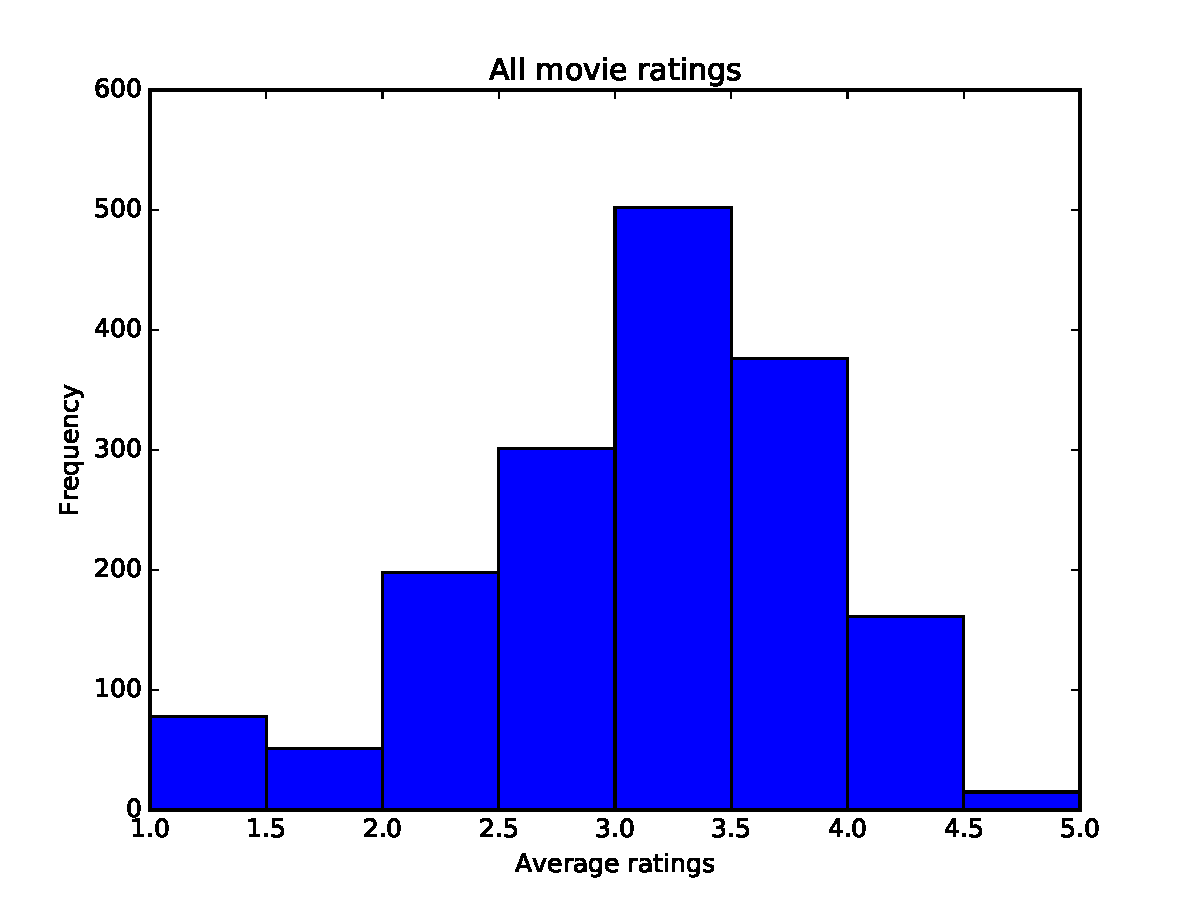
\includegraphics[width=\textwidth]{all_movie_ratings}
	\caption{All movie average ratings for in MovieLens.} \label{fig:all-movie}
\end{figure}


Figure \ref{fig:all-movie-sorted} provides another view of the average ratings for all movie in the MovieLens dataset. We can observe that the average ratings are integers when there are small numbers of ratings indicating that the average ratings may not be reliable.

\begin{figure}[H]
	\centering
	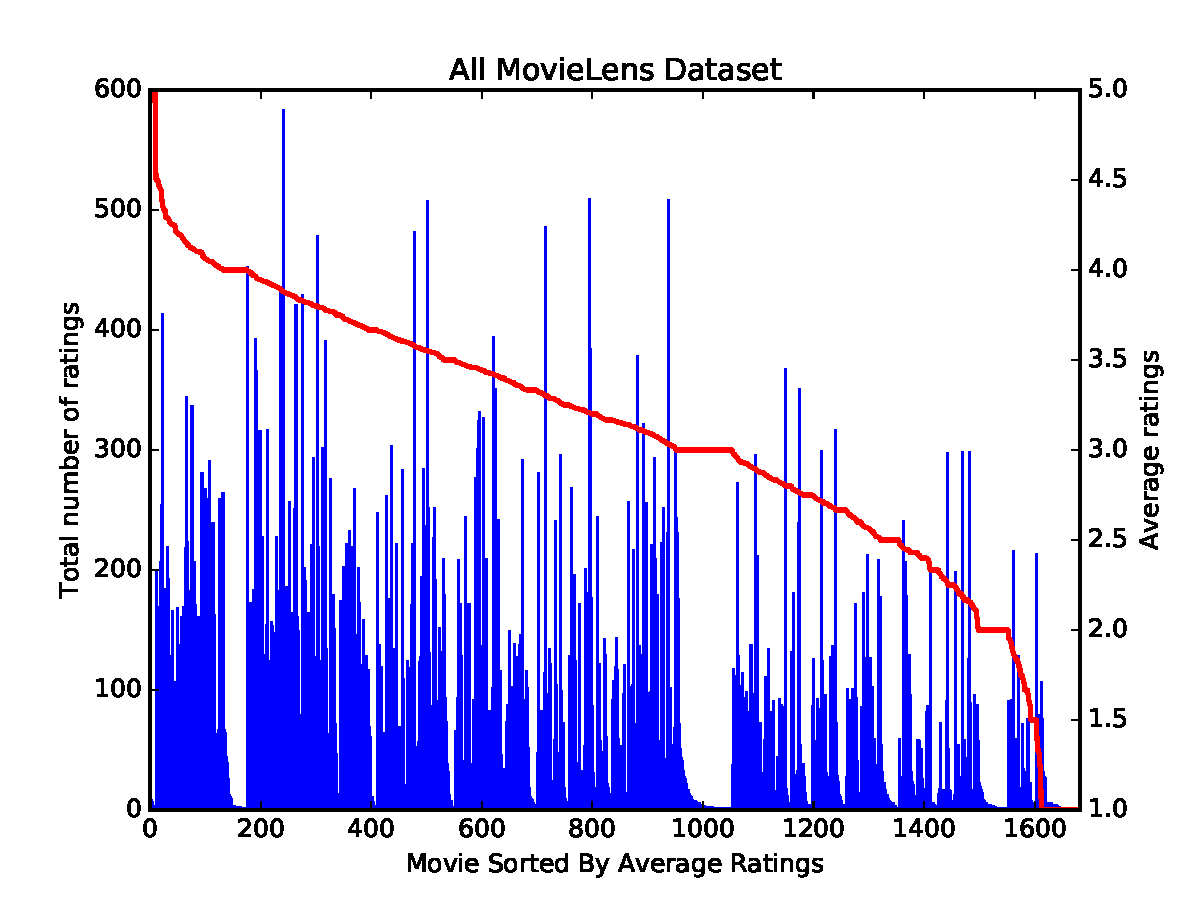
\includegraphics[width=\textwidth]{sorted_ratings}
	\caption{All movie average ratings for in MovieLens sorted according to the average ratings. Red line represents the average ratings, and blue bar charts represents the total number of ratings.} \label{fig:all-movie-sorted} 
\end{figure}

Figure \ref{fig:top-10-best} and \ref{fig:top-10-popular} shows distribution of ratings for the top 10 best movies and top 10 most popular movies respectively. First, we can see that the top 10 best movies have small numbers of ratings, but they are all 5 resulting in average ratings of 5. This observation indicates that the ratings are not too reliable. Second, the top most popular movies tend to have higher ratings. This observation indicates that a popular movie tends to be a good movie. It might also indicate that a good movie tends to be a popular movie. The causality is unclear, but good movies seem to be correlated to popular movies, making logical sense. 

\begin{figure}[H]
	\centering
	\subfloat[Top 10 best movies] {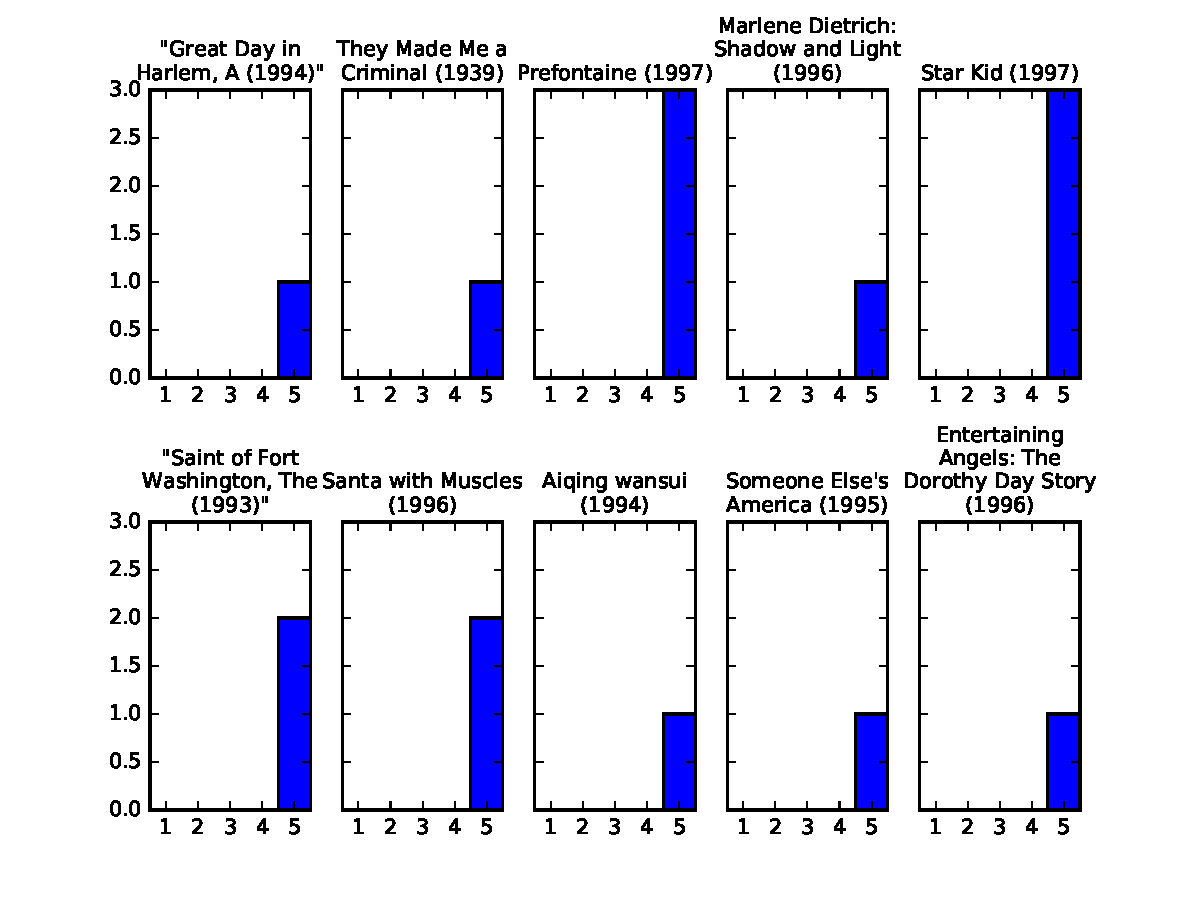
\includegraphics[width=0.8\textwidth, trim = 0cm 0mm 0cm 1cm, clip=true] {top_10_best_movie}\label{fig:top-10-best}}\\
	\subfloat[Top 10 most popular movies] {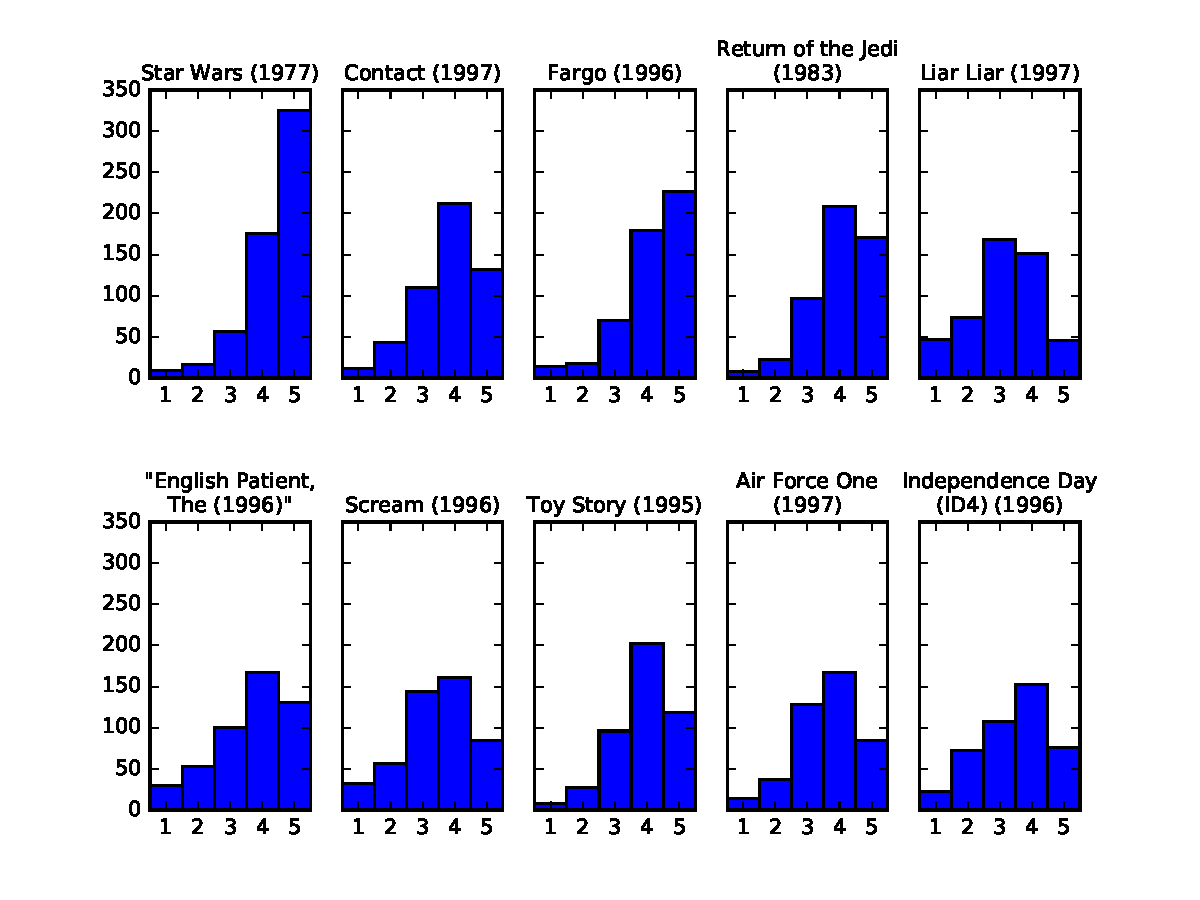
\includegraphics[width=0.8\textwidth, trim = 0cm 0mm 0cm 1.3cm, clip=true]{top_10_popular_movie}\label{fig:top-10-popular}}
	\caption{Ratings of top movies.} 
\end{figure}

Figure \ref{fig:average-3-genres} shows the average ratings of all movies in three different genres -- children, fantasy, and horror. There are less fantasy movies than children and horror. All three genres seems to have average ratings of about 2.5 to 3. The horror movies have a peak near average ratings of 2.5 to 3 and a small peak near average ratings of 1 to 1.5. This result indicates that horror movies are either really bad or average. The children movies are mostly average. The fantasy genre seems to have more movies with above average ratings than movies with below average ratings. The other two genres are more balanced.


\begin{figure}[H]
	\centering
	\subfloat[Children]{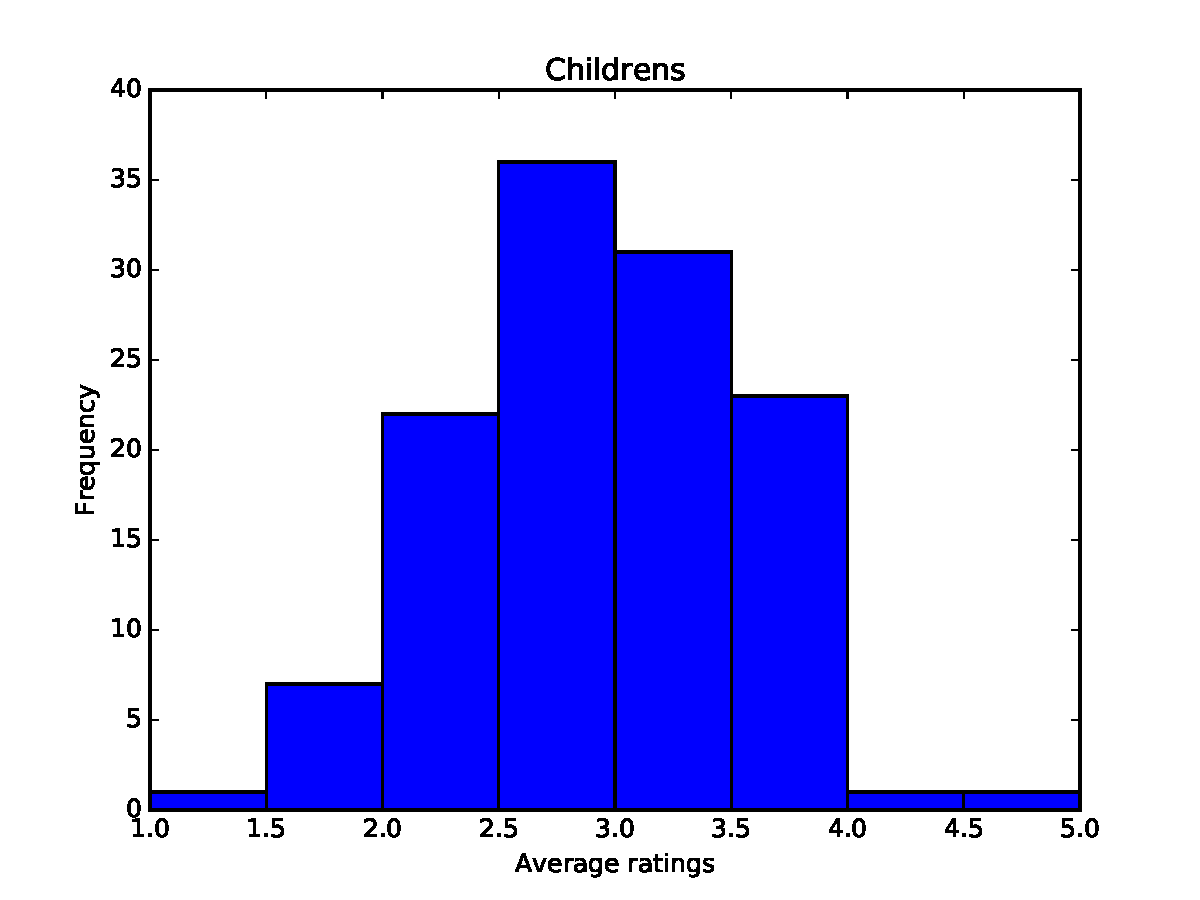
\includegraphics[width=0.33\textwidth, trim = 1cm 0mm 2cm 0mm, clip=true]{movie_genre_4}}
	\subfloat[Fantasy]{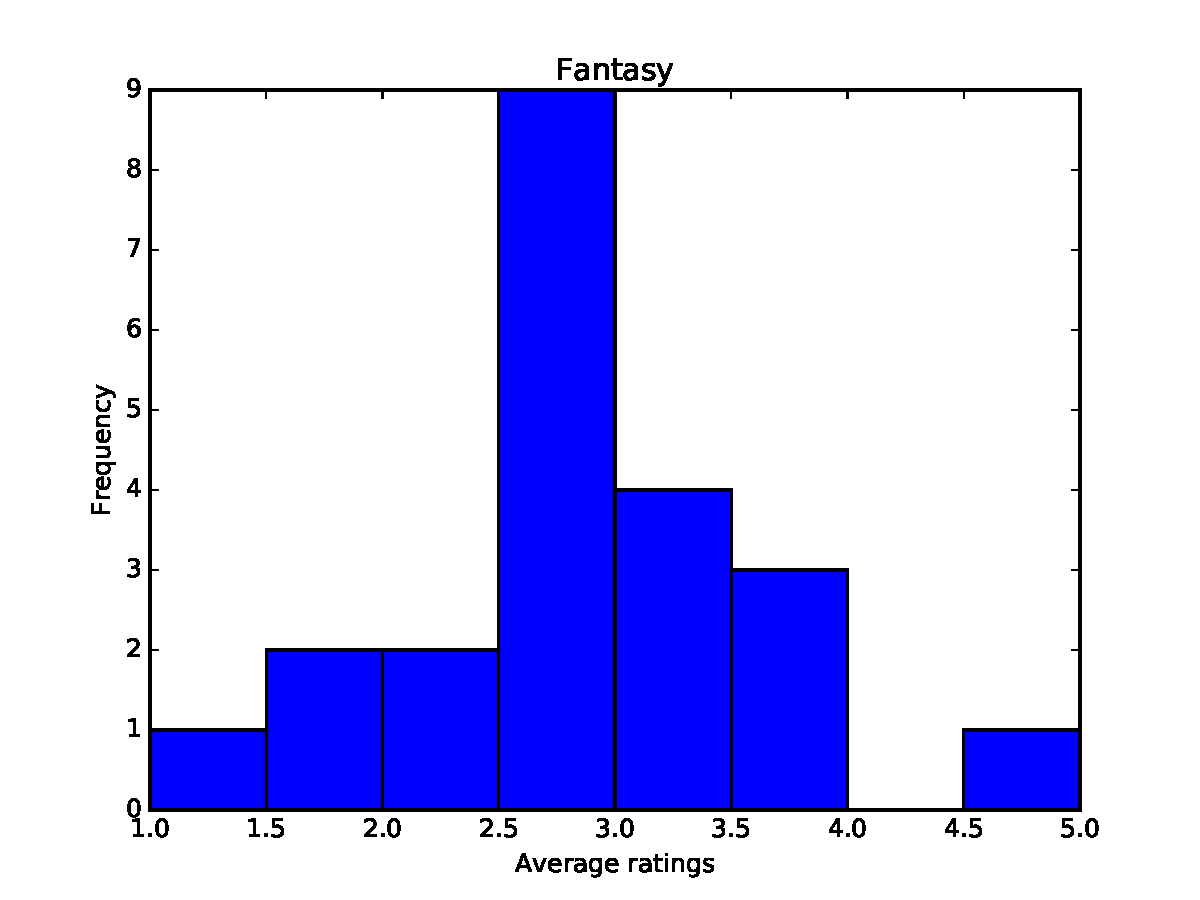
\includegraphics[width=0.33\textwidth, trim = 1cm 0mm 2cm 0mm, clip=true]{movie_genre_9}}
	\subfloat[Horror]{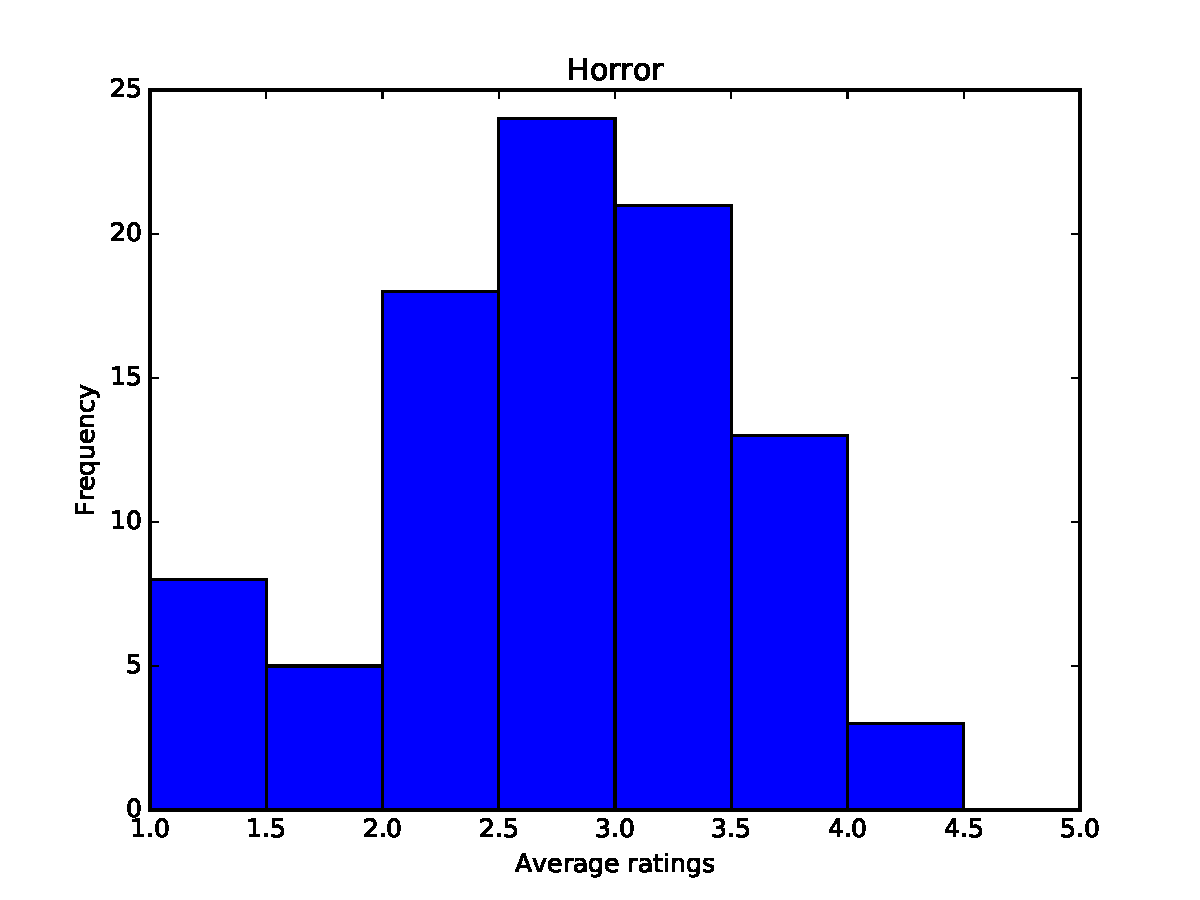
\includegraphics[width=0.33\textwidth, trim = 1cm 0mm 2cm 0mm, clip=true]{movie_genre_11}}
	\caption{Average ratings of all movies in three different genres.} \label{fig:average-3-genres}
\end{figure}
